% Options for packages loaded elsewhere
\PassOptionsToPackage{unicode}{hyperref}
\PassOptionsToPackage{hyphens}{url}
%
\documentclass[
]{book}
\title{Introduction to R and RStudio for Statistics Courses}
\author{William Murrah}
\date{2022-01-12}

\usepackage{amsmath,amssymb}
\usepackage{lmodern}
\usepackage{iftex}
\ifPDFTeX
  \usepackage[T1]{fontenc}
  \usepackage[utf8]{inputenc}
  \usepackage{textcomp} % provide euro and other symbols
\else % if luatex or xetex
  \usepackage{unicode-math}
  \defaultfontfeatures{Scale=MatchLowercase}
  \defaultfontfeatures[\rmfamily]{Ligatures=TeX,Scale=1}
\fi
% Use upquote if available, for straight quotes in verbatim environments
\IfFileExists{upquote.sty}{\usepackage{upquote}}{}
\IfFileExists{microtype.sty}{% use microtype if available
  \usepackage[]{microtype}
  \UseMicrotypeSet[protrusion]{basicmath} % disable protrusion for tt fonts
}{}
\makeatletter
\@ifundefined{KOMAClassName}{% if non-KOMA class
  \IfFileExists{parskip.sty}{%
    \usepackage{parskip}
  }{% else
    \setlength{\parindent}{0pt}
    \setlength{\parskip}{6pt plus 2pt minus 1pt}}
}{% if KOMA class
  \KOMAoptions{parskip=half}}
\makeatother
\usepackage{xcolor}
\IfFileExists{xurl.sty}{\usepackage{xurl}}{} % add URL line breaks if available
\IfFileExists{bookmark.sty}{\usepackage{bookmark}}{\usepackage{hyperref}}
\hypersetup{
  pdftitle={Introduction to R and RStudio for Statistics Courses},
  pdfauthor={William Murrah},
  hidelinks,
  pdfcreator={LaTeX via pandoc}}
\urlstyle{same} % disable monospaced font for URLs
\usepackage{color}
\usepackage{fancyvrb}
\newcommand{\VerbBar}{|}
\newcommand{\VERB}{\Verb[commandchars=\\\{\}]}
\DefineVerbatimEnvironment{Highlighting}{Verbatim}{commandchars=\\\{\}}
% Add ',fontsize=\small' for more characters per line
\usepackage{framed}
\definecolor{shadecolor}{RGB}{248,248,248}
\newenvironment{Shaded}{\begin{snugshade}}{\end{snugshade}}
\newcommand{\AlertTok}[1]{\textcolor[rgb]{0.94,0.16,0.16}{#1}}
\newcommand{\AnnotationTok}[1]{\textcolor[rgb]{0.56,0.35,0.01}{\textbf{\textit{#1}}}}
\newcommand{\AttributeTok}[1]{\textcolor[rgb]{0.77,0.63,0.00}{#1}}
\newcommand{\BaseNTok}[1]{\textcolor[rgb]{0.00,0.00,0.81}{#1}}
\newcommand{\BuiltInTok}[1]{#1}
\newcommand{\CharTok}[1]{\textcolor[rgb]{0.31,0.60,0.02}{#1}}
\newcommand{\CommentTok}[1]{\textcolor[rgb]{0.56,0.35,0.01}{\textit{#1}}}
\newcommand{\CommentVarTok}[1]{\textcolor[rgb]{0.56,0.35,0.01}{\textbf{\textit{#1}}}}
\newcommand{\ConstantTok}[1]{\textcolor[rgb]{0.00,0.00,0.00}{#1}}
\newcommand{\ControlFlowTok}[1]{\textcolor[rgb]{0.13,0.29,0.53}{\textbf{#1}}}
\newcommand{\DataTypeTok}[1]{\textcolor[rgb]{0.13,0.29,0.53}{#1}}
\newcommand{\DecValTok}[1]{\textcolor[rgb]{0.00,0.00,0.81}{#1}}
\newcommand{\DocumentationTok}[1]{\textcolor[rgb]{0.56,0.35,0.01}{\textbf{\textit{#1}}}}
\newcommand{\ErrorTok}[1]{\textcolor[rgb]{0.64,0.00,0.00}{\textbf{#1}}}
\newcommand{\ExtensionTok}[1]{#1}
\newcommand{\FloatTok}[1]{\textcolor[rgb]{0.00,0.00,0.81}{#1}}
\newcommand{\FunctionTok}[1]{\textcolor[rgb]{0.00,0.00,0.00}{#1}}
\newcommand{\ImportTok}[1]{#1}
\newcommand{\InformationTok}[1]{\textcolor[rgb]{0.56,0.35,0.01}{\textbf{\textit{#1}}}}
\newcommand{\KeywordTok}[1]{\textcolor[rgb]{0.13,0.29,0.53}{\textbf{#1}}}
\newcommand{\NormalTok}[1]{#1}
\newcommand{\OperatorTok}[1]{\textcolor[rgb]{0.81,0.36,0.00}{\textbf{#1}}}
\newcommand{\OtherTok}[1]{\textcolor[rgb]{0.56,0.35,0.01}{#1}}
\newcommand{\PreprocessorTok}[1]{\textcolor[rgb]{0.56,0.35,0.01}{\textit{#1}}}
\newcommand{\RegionMarkerTok}[1]{#1}
\newcommand{\SpecialCharTok}[1]{\textcolor[rgb]{0.00,0.00,0.00}{#1}}
\newcommand{\SpecialStringTok}[1]{\textcolor[rgb]{0.31,0.60,0.02}{#1}}
\newcommand{\StringTok}[1]{\textcolor[rgb]{0.31,0.60,0.02}{#1}}
\newcommand{\VariableTok}[1]{\textcolor[rgb]{0.00,0.00,0.00}{#1}}
\newcommand{\VerbatimStringTok}[1]{\textcolor[rgb]{0.31,0.60,0.02}{#1}}
\newcommand{\WarningTok}[1]{\textcolor[rgb]{0.56,0.35,0.01}{\textbf{\textit{#1}}}}
\usepackage{longtable,booktabs,array}
\usepackage{calc} % for calculating minipage widths
% Correct order of tables after \paragraph or \subparagraph
\usepackage{etoolbox}
\makeatletter
\patchcmd\longtable{\par}{\if@noskipsec\mbox{}\fi\par}{}{}
\makeatother
% Allow footnotes in longtable head/foot
\IfFileExists{footnotehyper.sty}{\usepackage{footnotehyper}}{\usepackage{footnote}}
\makesavenoteenv{longtable}
\usepackage{graphicx}
\makeatletter
\def\maxwidth{\ifdim\Gin@nat@width>\linewidth\linewidth\else\Gin@nat@width\fi}
\def\maxheight{\ifdim\Gin@nat@height>\textheight\textheight\else\Gin@nat@height\fi}
\makeatother
% Scale images if necessary, so that they will not overflow the page
% margins by default, and it is still possible to overwrite the defaults
% using explicit options in \includegraphics[width, height, ...]{}
\setkeys{Gin}{width=\maxwidth,height=\maxheight,keepaspectratio}
% Set default figure placement to htbp
\makeatletter
\def\fps@figure{htbp}
\makeatother
\setlength{\emergencystretch}{3em} % prevent overfull lines
\providecommand{\tightlist}{%
  \setlength{\itemsep}{0pt}\setlength{\parskip}{0pt}}
\setcounter{secnumdepth}{5}
\usepackage{booktabs}
\ifLuaTeX
  \usepackage{selnolig}  % disable illegal ligatures
\fi
\usepackage[]{natbib}
\bibliographystyle{plainnat}

\begin{document}
\maketitle

{
\setcounter{tocdepth}{1}
\tableofcontents
}
\hypertarget{preface}{%
\chapter*{Preface}\label{preface}}
\addcontentsline{toc}{chapter}{Preface}

This notebook exists to help people get started using R and RStudio for data analysis and statistics.
It is a work-in-progress, but should contain instructions, examples, and links to videos useful to those interested in using the R programming language.

\hypertarget{intro}{%
\chapter{Why R and RStudio?}\label{intro}}

Chapter justifying the use of R and RStudio

\hypertarget{why-r-and-not-another-statistical-program}{%
\section{Why R and Not Another Statistical Program?}\label{why-r-and-not-another-statistical-program}}

\hypertarget{statistical-programs-versus-statistical-programming-language}{%
\subsection{Statistical Programs versus Statistical Programming Language}\label{statistical-programs-versus-statistical-programming-language}}

\begin{itemize}
\tightlist
\item
  Statistical Programs

  \begin{itemize}
  \tightlist
  \item
    fixed menus
  \item
    limited procedures (at least in the menus)
  \item
    leads to compartmentalizing models (e.g.~ANOVA, regression, GLM)
  \end{itemize}
\item
  Statistical Programming Languages (SPLs)

  \begin{itemize}
  \tightlist
  \item
    Turing complete: if you can create an algorithm you can program it
  \item
    Very flexible
  \item
    Integration of models: One model to rule them all!
  \end{itemize}
\end{itemize}

R is a statistical programming language, which means it is a programming language designed specifically to do statistics.

\hypertarget{install}{%
\chapter{Installing R and RStudio}\label{install}}

Installing software.

\hypertarget{objectives}{%
\section{Objectives}\label{objectives}}

The goal of this chapter is to get you up and running with the R statistical programming language and the RStudio integrated development environment.

If you are reading this because you are taking one of my courses, you must decide how you want to use R and RStudio for the course.
You have two basic options:

\begin{enumerate}
\def\labelenumi{\arabic{enumi}.}
\tightlist
\item
  you can install them on your own computer, or
\item
  you can use Auburn Universities education virtual lab (VLab), online.
\end{enumerate}

If you have a computer that you will be using consistently for this course, I recommend installing R and RStudio on that computer.
Both are free and will be much easier to use if you install them directly on your computer.
If you have decided to install the software on your computer you can skip to the following video.
Note, that you must be a student within the university, and have DUO setup to use VLab.
If you think you want to use the virtual lab, watch this video:

\href{https://nv.instructuremedia.com/fetch/QkFoYkIxc0hhUVNIRGFrSE1Hd3JCeWhUREdFPS0tZjk4ODFlYWEyZWFiNWQwYWYyZDk0YTZjMjljZTJlMjBkNmIwMzE5Yw.mp4}{Using VLab to acces R/RStudio}

\hypertarget{installing-r}{%
\section{Installing R}\label{installing-r}}

\hypertarget{installing-rstudio}{%
\section{Installing RStudio}\label{installing-rstudio}}

\hypertarget{tour}{%
\chapter{A Tour of R and RStudio}\label{tour}}

Learn the basics of using R and RStudio

\hypertarget{raspl}{%
\chapter{R As a Statistical Programming Language}\label{raspl}}

This chapter describes R as a statistical programming language to give you some basic concepts to understand how R works.
Such concepts will hopefully help you organize what you are learning about R.
This is important because you will not be able to memorize all of the things you need to do to use R.
But, having some general concepts to hang what you are learning on, should help you build a solid skill foundation.
This explanation will be a gross oversimplification of R, but it should be a good starting model of R that you can build on as you master the language.

\hypertarget{elements-of-statistical-programming}{%
\section{Elements of Statistical Programming}\label{elements-of-statistical-programming}}

An object is a thing that has one or more \emph{states}, and one or more \emph{behaviors.}
Take for example you cell phone.
It has many states, such as on or off, and many behaviors, such as making phone calls, sending texts, or surfing the web.
\textbf{Everything in R is an object}.
Objects in R are very similar to objects like your cell phone, in that they have states and behaviors.
Our goal is to learn how to use these objects to help us do science.

There are basically two types of objects in R: \textbf{data objects} and \textbf{function objects}.
Data objects store information, while function objects process or manipulate information.

\hypertarget{expressions}{%
\subsection{Expressions}\label{expressions}}

We use objects in R through \textbf{expressions}.
An expression is simply a combination of objects that R can evaluate.
So, we type something into R, R processes it and gives us the results.
For example, if we type \texttt{1\ +\ 2} into the R console, it will give us the result \texttt{3}:

\begin{Shaded}
\begin{Highlighting}[]
\DecValTok{1} \SpecialCharTok{+} \DecValTok{2}
\end{Highlighting}
\end{Shaded}

\begin{verbatim}
[1] 3
\end{verbatim}

So, expressions are simply objects or combinations of objects submitted to R in a way R can evaluate them.

\hypertarget{basic-elements-of-a-good-spl}{%
\subsection{Basic Elements of a Good SPL}\label{basic-elements-of-a-good-spl}}

\begin{enumerate}
\def\labelenumi{\arabic{enumi}.}
\tightlist
\item
  a rich set of \textbf{primitive expressions}
\item
  mechanisms for \textbf{combining expressions} into more complex expressions
\item
  means of \textbf{abstraction}, which allow for naming and manipulating compound objects
\end{enumerate}

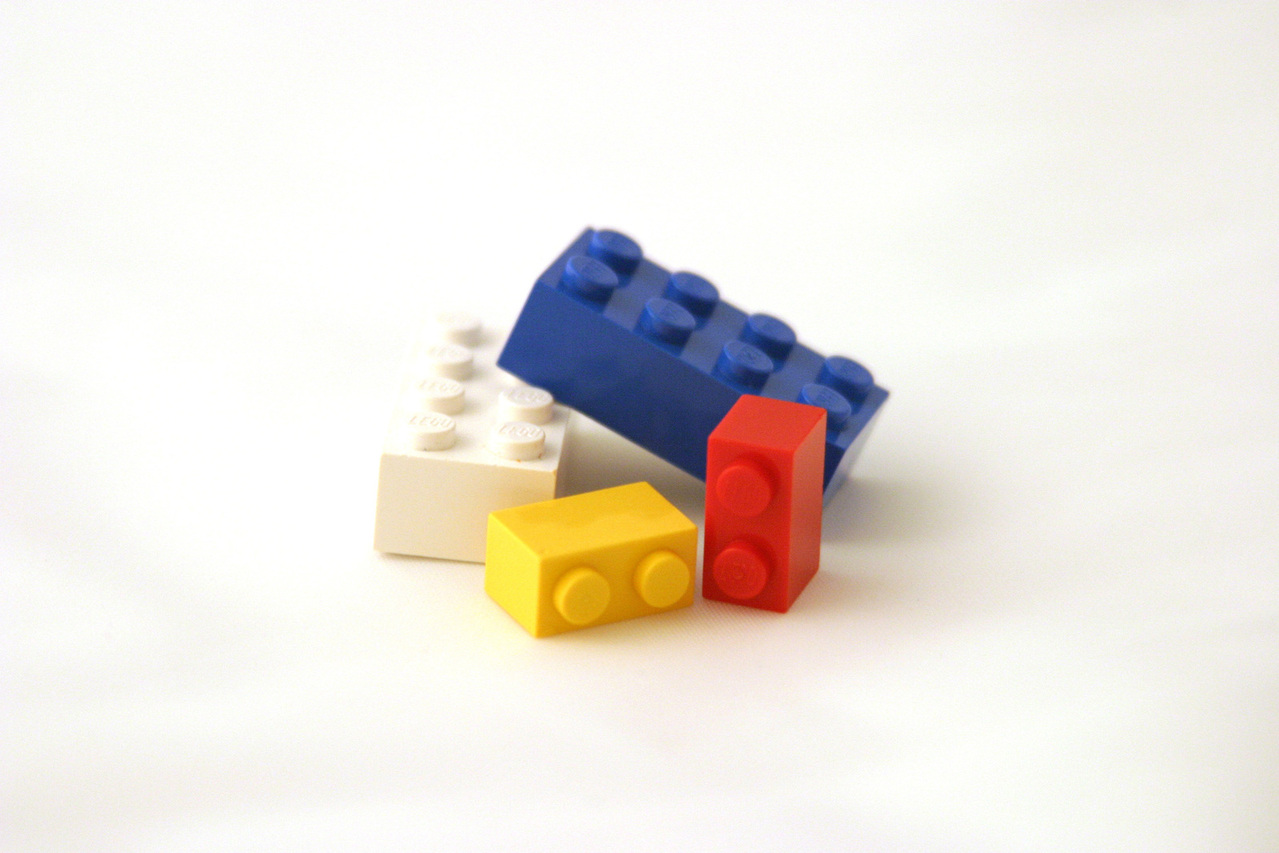
\includegraphics[width=0.4\linewidth]{figures/blocks}

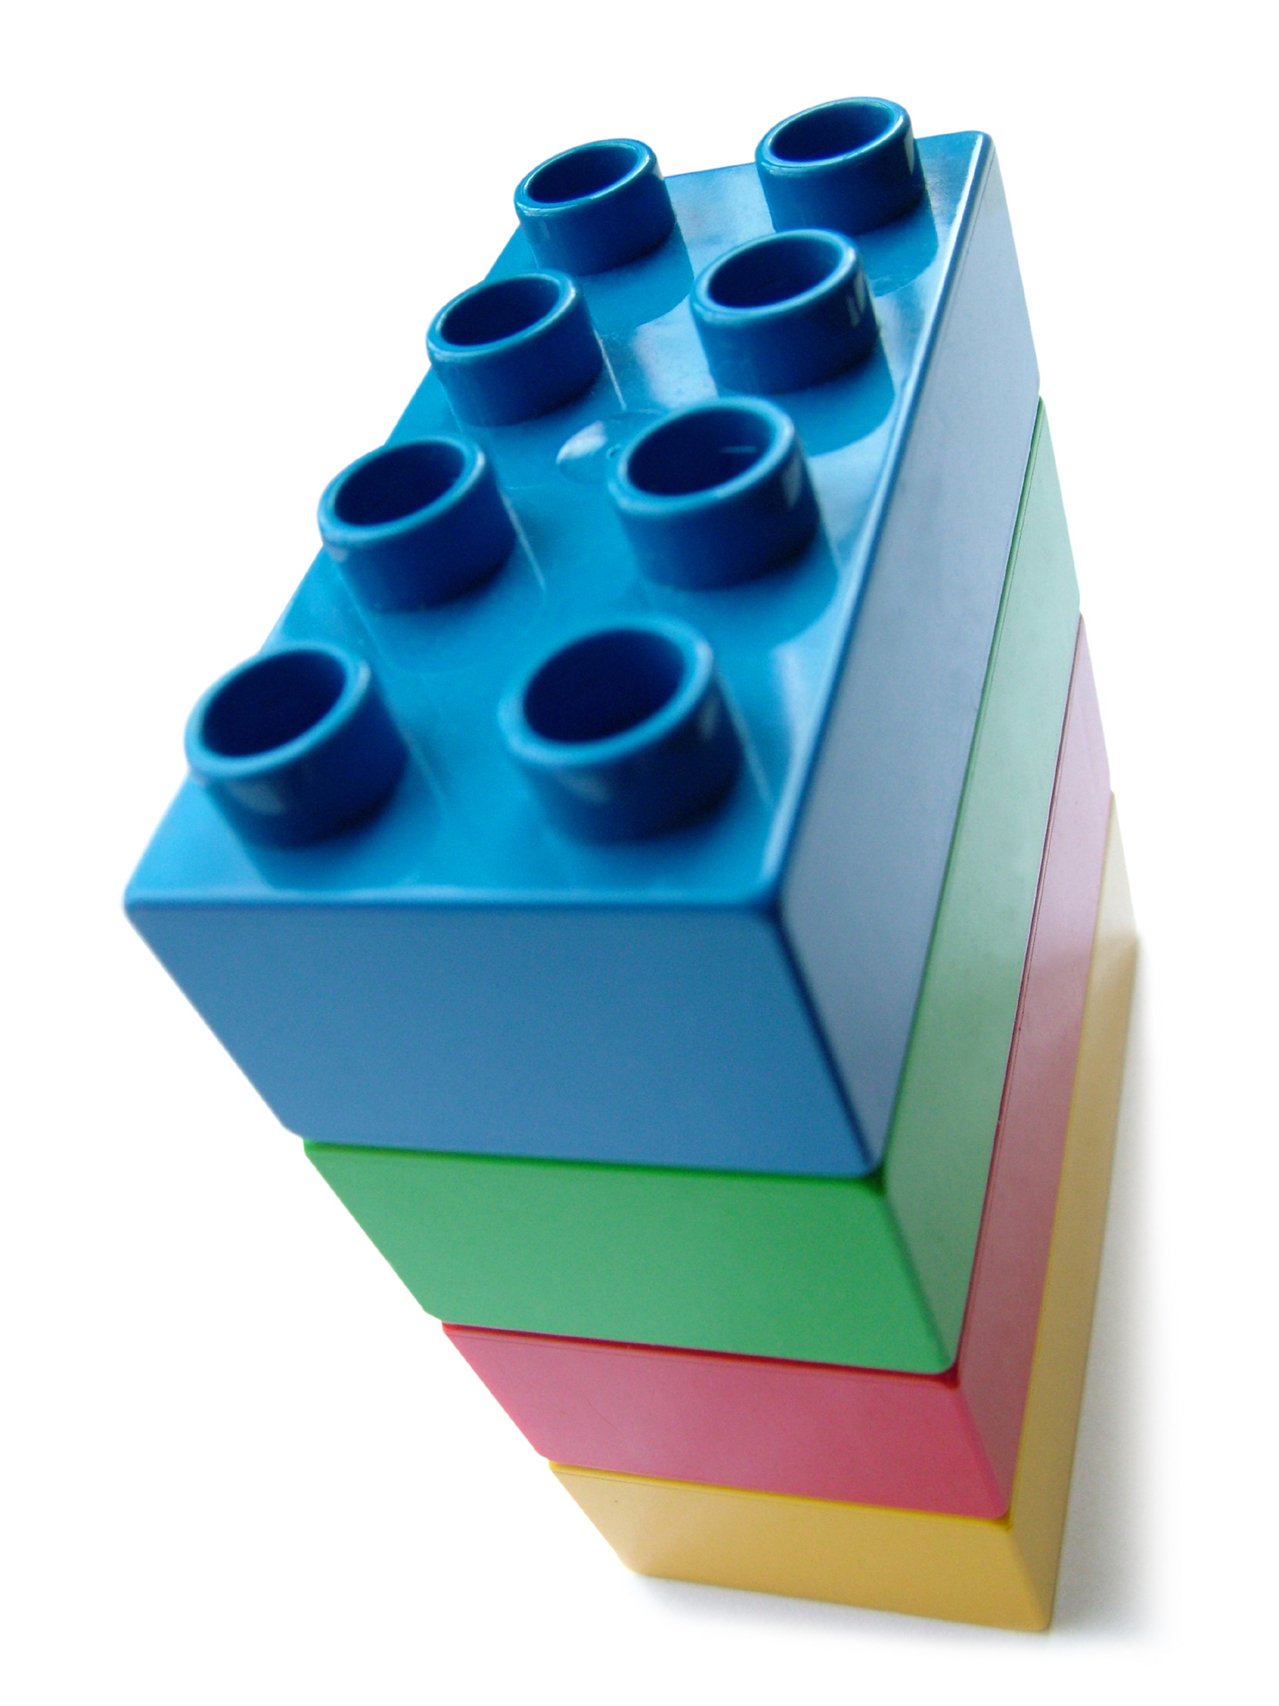
\includegraphics[width=0.2\linewidth]{figures/blockstack}

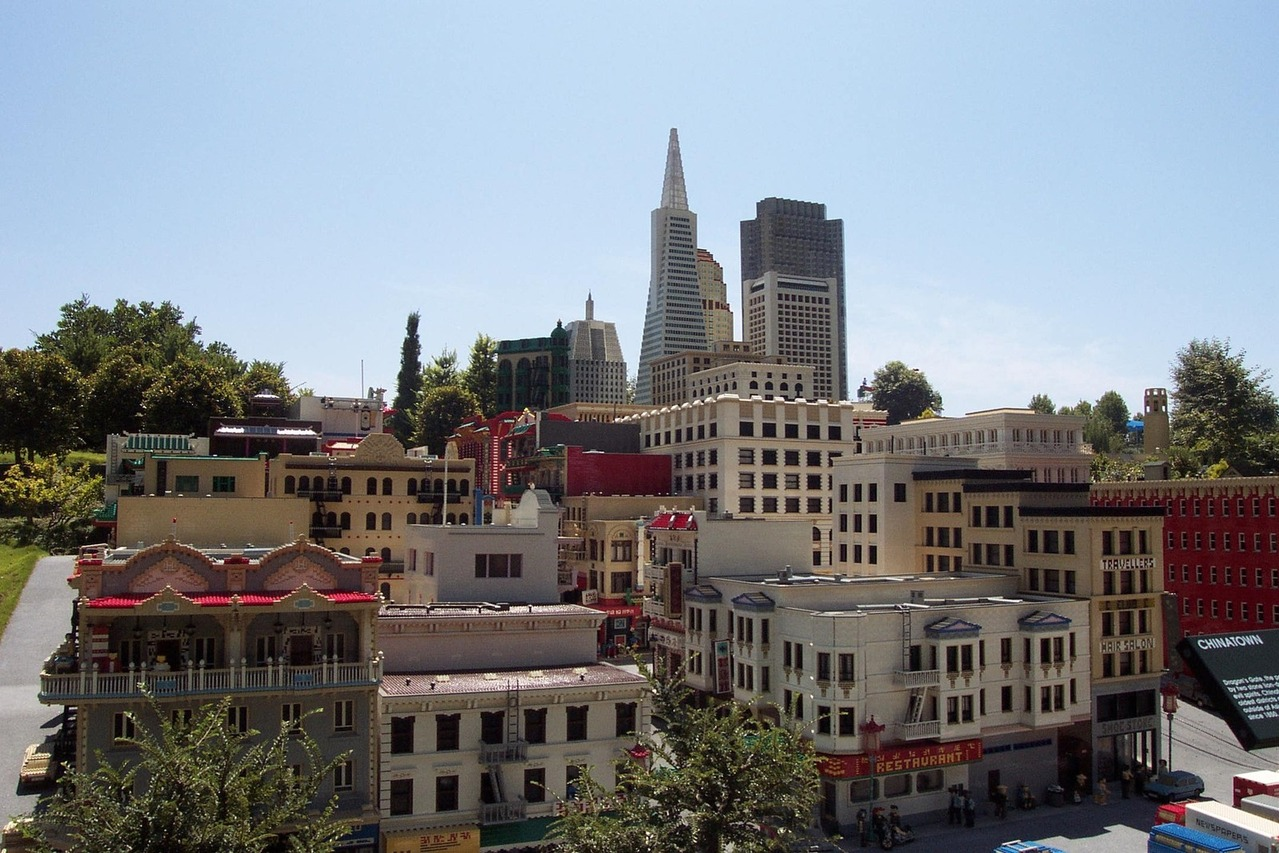
\includegraphics[width=0.4\linewidth]{figures/sanfran}

\hypertarget{primitive-expressions}{%
\section{Primitive Expressions}\label{primitive-expressions}}

\begin{itemize}
\item
  Everything in R is an object
\item
  Primitive objects are the simplest elements of a programming language, and include:

  \begin{itemize}
  \tightlist
  \item
    \emph{primitive data}
  \item
    \emph{primitive functions}
  \end{itemize}
\item
  They can be thought of as the basic building blocks for everything else in the language.
\item
  An \textbf{expression} is an input that the programming language can evaluate, and consists of function and data objects.
\end{itemize}

\hypertarget{primitive-data-types}{%
\section{Primitive Data Types:}\label{primitive-data-types}}

Data objects are the primary means of storing information in R.
R has a few basic \emph{data types}:

\begin{itemize}
\item
  \textbf{Numeric} -

  \begin{itemize}
  \tightlist
  \item
    \texttt{numeric}

    \begin{itemize}
    \tightlist
    \item
      \texttt{int} - integers (\texttt{1,2})
    \item
      \texttt{num} - real number (\texttt{1.2,\ -3.1,\ 200.0})
    \end{itemize}
  \end{itemize}
\item
  \textbf{character} or \textbf{string} -

  \begin{itemize}
  \tightlist
  \item
    \texttt{character}

    \begin{itemize}
    \tightlist
    \item
      \texttt{"Hello\ world!"}, \texttt{"Ten"}, \texttt{\textquotesingle{}Cat\textquotesingle{}}
    \item
      \texttt{"This\ is\ a\ sentence,\ which\ is\ a\ string"}
    \item
      \texttt{"10"} ( in single or double quotes, as long as they match)
    \end{itemize}
  \end{itemize}
\item
  \textbf{Boolean} or \textbf{Logical}

  \begin{itemize}
  \tightlist
  \item
    \texttt{logical}

    \begin{itemize}
    \tightlist
    \item
      \texttt{TRUE} or \texttt{FALSE} (use operators such as \emph{or}, \emph{and} and \emph{not}).
    \item
      They will evaluate to numbers where \texttt{FALSE} evaluates to zero, and \texttt{TRUE} evaluates to one.
    \item
      For example. if you enter \texttt{TRUE\ +\ 1} you will get \texttt{2} in return.
    \end{itemize}
  \end{itemize}
\end{itemize}

\begin{Shaded}
\begin{Highlighting}[]
\FunctionTok{mode}\NormalTok{(}\ConstantTok{TRUE}\NormalTok{)}
\end{Highlighting}
\end{Shaded}

\begin{verbatim}
[1] "logical"
\end{verbatim}

\begin{Shaded}
\begin{Highlighting}[]
\ConstantTok{TRUE} \SpecialCharTok{+} \DecValTok{1}
\end{Highlighting}
\end{Shaded}

\begin{verbatim}
[1] 2
\end{verbatim}

\hypertarget{primitive-functions}{%
\section{Primitive Functions}\label{primitive-functions}}

R uses functions to do all computations.

\hypertarget{operators}{%
\subsection{Operators}\label{operators}}

\begin{itemize}
\tightlist
\item
  Arithmetic Operators

  \begin{itemize}
  \tightlist
  \item
    \texttt{+}, \texttt{-}, \texttt{*}, \texttt{/}, \texttt{\^{}}
  \end{itemize}
\item
  Comparison (also called Boolean, Logical or Predicate) Operators

  \begin{itemize}
  \tightlist
  \item
    \texttt{\textless{}},\texttt{\textgreater{}},\texttt{==}, \texttt{\textless{}=}, \texttt{\textgreater{}=}, \texttt{!=}
  \item
    less than, greater than, equal to, less than or equal to, greater than or equal to, not equal to
  \item
    return \texttt{TRUE} or \texttt{FALSE}
  \end{itemize}
\item
  Logical Operator

  \begin{itemize}
  \tightlist
  \item
    \texttt{\&}, \texttt{\textbar{}} ,\texttt{!}
  \item
    also return \texttt{TRUE} or \texttt{FALSE}
  \end{itemize}
\item
  Other functions

  \begin{itemize}
  \tightlist
  \item
    \texttt{mode()}
  \item
    \texttt{length()}
  \item
    \texttt{sum()}
  \item
    \texttt{sqrt()}
  \item
    \texttt{log()}
  \item
    \texttt{exp()}
  \end{itemize}
\item
  Assignment operators (assignment will be discussed below)

  \begin{itemize}
  \tightlist
  \item
    \texttt{\textless{}-} \textbf{preferred assignment operator - always use this one}
  \item
    \texttt{=} this will also work, but can be confusing (note different from \texttt{==}, the comparison operator)
  \item
    \texttt{-\textgreater{}} is also an assignment operator, but we will not use it.
  \end{itemize}
\end{itemize}

\hypertarget{programming-languages-are-not-forgiving}{%
\section{Programming Languages are Not Forgiving}\label{programming-languages-are-not-forgiving}}

\hypertarget{syntactically-valid-expressions}{%
\subsection{Syntactically valid expressions}\label{syntactically-valid-expressions}}

Expressions must be syntactically valid.

\begin{itemize}
\tightlist
\item
  syntax (form)

  \begin{itemize}
  \tightlist
  \item
    English: ``cat dog boy'' - not syntactically valid
  \item
    English: ``cat hugs boy'' - syntactically valid
  \end{itemize}
\item
  programming language:

  \begin{itemize}
  \tightlist
  \item
    ``hi'' 5 - not syntactically valid
  \item
    3.2*5 - syntactically valid
  \end{itemize}
\end{itemize}

\hypertarget{semantically-valid-expressions}{%
\subsection{Semantically valid expressions}\label{semantically-valid-expressions}}

\begin{itemize}
\tightlist
\item
  semantics - (meaning)

  \begin{itemize}
  \tightlist
  \item
    English: ``I are hungry'' - syntactically valid but semantic error
  \item
    programming language:

    \begin{itemize}
    \tightlist
    \item
      3 + ``hi'' - semantic error (you can't use addition on character strings)
    \end{itemize}
  \end{itemize}
\item
  Chomsky:
  ``colorless green ideas sleep furiously''
\end{itemize}

This statement is syntactically valid, but does not make sense, so makes a semantic error.

\textbf{In R you have to combine expressions in a way that R ``understands'' and this combination should be meaningful}.

\hypertarget{assignment}{%
\section{Assignment}\label{assignment}}

We will often want to save data in a variable. We can do that with \textbf{assignment}, which utilizes an assignment operator.

\begin{Shaded}
\begin{Highlighting}[]
\NormalTok{x }\OtherTok{\textless{}{-}} \DecValTok{2}
\end{Highlighting}
\end{Shaded}

\begin{Shaded}
\begin{Highlighting}[]
\NormalTok{x}
\end{Highlighting}
\end{Shaded}

\begin{verbatim}
[1] 2
\end{verbatim}

\begin{Shaded}
\begin{Highlighting}[]
\NormalTok{pet }\OtherTok{\textless{}{-}} \StringTok{"dog"}
\end{Highlighting}
\end{Shaded}

\begin{Shaded}
\begin{Highlighting}[]
\NormalTok{pet}
\end{Highlighting}
\end{Shaded}

\begin{verbatim}
[1] "dog"
\end{verbatim}

Assignments are special expressions that are composed of three parts, a \textbf{name}, an \textbf{assignment operator}, and an \textbf{expression}.

For the following assignment,

\begin{Shaded}
\begin{Highlighting}[]
\NormalTok{x }\OtherTok{\textless{}{-}} \DecValTok{1}\SpecialCharTok{:}\DecValTok{10}
\end{Highlighting}
\end{Shaded}

\texttt{x} is the name, \texttt{\textless{}-} is the assignment operator, and \texttt{1:10} is an expression.
Names in R can be anything that includes letters, numbers, a period (\texttt{.}) or an underscore (\texttt{\_}), as long as it begins with either a letter or a period.
Here are some valid, followed by invalid names

\begin{Shaded}
\begin{Highlighting}[]
\CommentTok{\# Valid}
\NormalTok{IQ}
\NormalTok{c3p0}
\NormalTok{Height\_inches}
\NormalTok{weight.lbs}
\NormalTok{.hidden}

\CommentTok{\# Invalid (you will get an error message)}
\NormalTok{\_cat}
\NormalTok{1dog}
\NormalTok{\%sales}
\NormalTok{Heigth}\SpecialCharTok{{-}}\NormalTok{Inches}
\end{Highlighting}
\end{Shaded}

There are also some names that cannot be used because they are names of primitive R objects (e.g.~\texttt{if}, \texttt{for}, \texttt{else}, \texttt{in}).
Type \texttt{?reserved} in the R console for a complete list.

There are at least three assignment operators, as mentioned above, but it is commonly recommended that you use \texttt{\textless{}-}, because it makes clear that you are taking some expression and putting it in an object.
So we would say of the assignment of \texttt{x\ \textless{}-\ 1:10} that x gets the integers 1 through 10, suggesting that we are putting the integers into the object \texttt{x}.

Just about any expression can be passed to a name with the assignment operator.

\hypertarget{combining-expressions}{%
\section{Combining Expressions}\label{combining-expressions}}

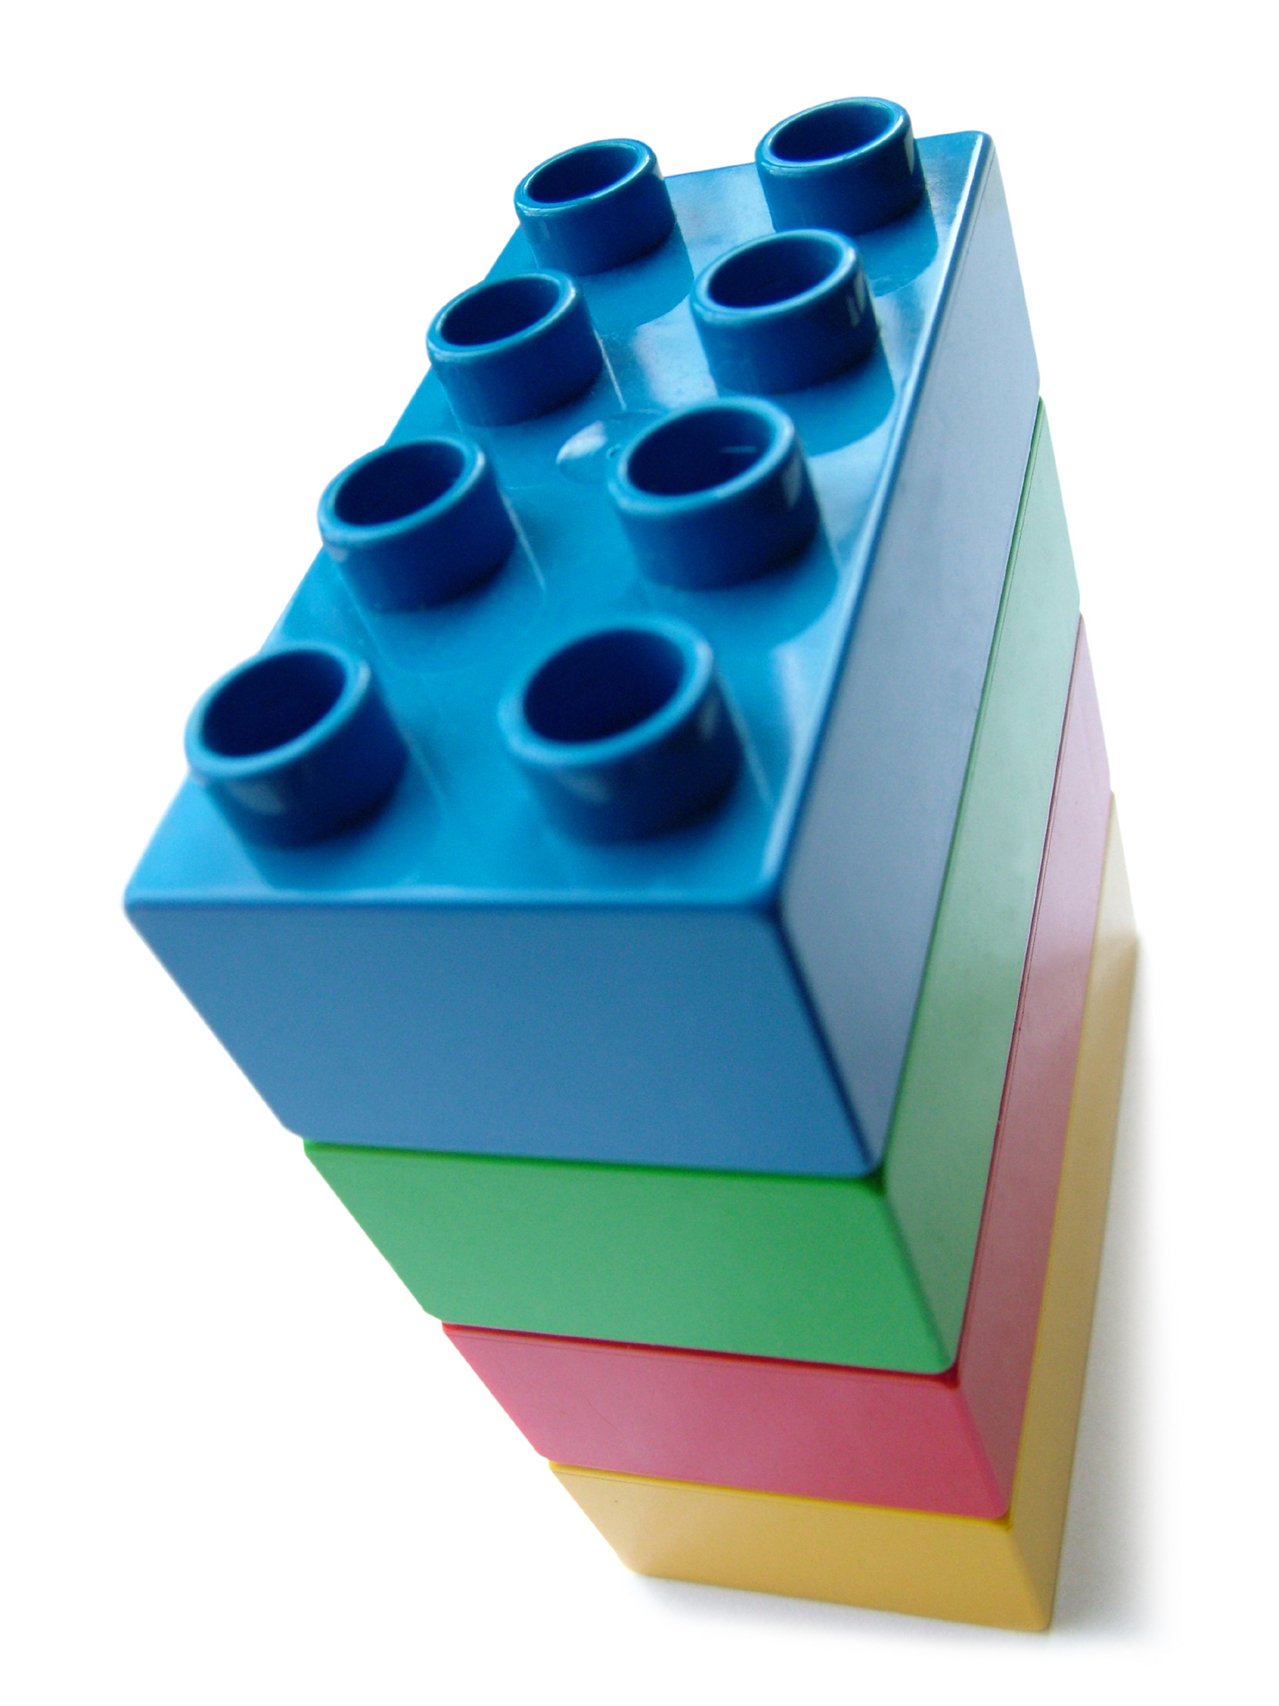
\includegraphics[width=0.3\linewidth]{figures/blockstack}

\hypertarget{complex-data-types}{%
\section{Complex Data Types}\label{complex-data-types}}

\begin{itemize}
\tightlist
\item
  Scalars, Vectors, Matrices, and Arrays
\item
  Lists
\item
  Dataframes
\end{itemize}

\hypertarget{grouping-homogeneous-data-types}{%
\section{Grouping Homogeneous Data Types}\label{grouping-homogeneous-data-types}}

\begin{itemize}
\tightlist
\item
  combining scalars
\end{itemize}

\begin{verbatim}
c()
\end{verbatim}

\begin{itemize}
\tightlist
\item
  combining expressions
\end{itemize}

\begin{verbatim}
{}
\end{verbatim}

\begin{itemize}
\tightlist
\item
  combining vectors
\end{itemize}

\begin{verbatim}
cbind()
rbind()
\end{verbatim}

\hypertarget{complex-functions}{%
\section{Complex Functions}\label{complex-functions}}

\begin{itemize}
\tightlist
\item
  Vectorization
\item
  Nested Functions
\item
  Loops and Conditional execution
\end{itemize}

\hypertarget{abstraction}{%
\section{Abstraction}\label{abstraction}}

\begin{itemize}
\tightlist
\item
  Assignment
\item
\end{itemize}

\hypertarget{data-abstraction}{%
\section{Data Abstraction}\label{data-abstraction}}

\hypertarget{functional-abstraction}{%
\section{Functional Abstraction}\label{functional-abstraction}}

\hypertarget{anatomy-of-a-function}{%
\section{Anatomy of a Function}\label{anatomy-of-a-function}}

\begin{verbatim}
name <- function(arg_1, arg_2, ...) {
    expression_1
    expression_2
    ...
    output <- expression_3
    return(output)
}
\end{verbatim}

\hypertarget{files-directories-and-projects}{%
\chapter{Files, Directories, and Projects}\label{files-directories-and-projects}}

\href{https://auburn.hosted.panopto.com/Panopto/Pages/Viewer.aspx?id=48773598-f6ba-4771-8515-ad880135ee36}{File Navigation in RStudio}

\href{https://auburn.hosted.panopto.com/Panopto/Pages/Viewer.aspx?id=aed0e2a9-004f-453f-80c7-abbe010a063b}{Organizing Projects in RStudio}

  \bibliography{book.bib,packages.bib}

\end{document}
